\documentclass[7pt]{article}
\twocolumn
\usepackage[utf8]{inputenc}
\usepackage{graphicx}
\usepackage{subcaption}
\usepackage{caption}
\usepackage{siunitx}
\usepackage{hyperref}
\graphicspath{{./images/}}
\usepackage{amsmath}
\usepackage{amsfonts}
\usepackage[version=4]{mhchem}

\usepackage[a4paper, total={183mm, 247mm}]{geometry}
\usepackage[switch]{lineno}
\linenumbers

\bibliographystyle{unsrt}
\usepackage[superscript,biblabel]{cite}

\newcommand*{\ts}{{\tau^{*}}}
\newcommand*{\diff}{\mathop{}\!\mathrm{d}}
\newcommand{\ps}{\si{\pico\second}}
\newcommand{\ns}{\si{\nano\second}}
\newcommand{\fs}{\si{\femto\second}}
\newcommand{\ips}{\si{\per\pico\second}}
\newcommand{\us}{\si{\micro\second}} 
\newcommand{\iA}{\si{\per\angstrom}}
\newcommand{\K}{\si{\kelvin}} 
\newcommand{\amu}{\si{\amu}} 
\newcommand{\uzeta}{\si{\pico\second\per\angstrom\squared}}
\newcommand{\THz}{\si{\tera\hertz}}

\usepackage{sectsty}
\sectionfont{\small}
\subsectionfont{\small}

\title{Justification for the use of Markovian Langevin statistics in the modeling of activated surface diffusion.}

\date{September 2021}

\begin{document}

\maketitle

Abstract max length: 200 words

\section*{Abstract 1 (239)}

At low temperatures, the motion of an adatom across a surface is an activated diffusion process characterized by the rate of hopping between adsorption sites. An understanding of what properties influence a system's hopping rate, and how these emerge from microscopic motion, allow for the classification and development of materials with desirable transport properties. The standard approach to modeling surface dynamics via the two dimensional Markovian Langevin equation leads to the classification of systems through the properties of the potential, such as an activation energy, and a single interaction strength parameter. The consequences of modeling a complex band-limited system with linear Markovian forces is not fully understood and it is unclear whether more parameters are required to fully characterize such systems. Through the study of four distinct models of microscopic motion covering correlated noise, alternative models of friction, and motion in three dimensions, we show that the two dimensional equilibrium phase space distribution and the total energy decorrelation rate are enough to constrain the hopping rate and jump distributions of an adatom to within a few percent. Our results validate the standard approach in the field provided the Markovian interaction strength parameter is reinterpreted as an effective energy exchange rate to which many effects contribute. Insights gained into the mechanisms of energy exchange suggest noise correlations have a strong effect on the hopping pre-exponential factor of systems where lateral adatom vibration frequencies are comparable to the phonon cutoff frequency.  

\section*{Abstract 2 (202)}

Low temperature surface diffusion is driven by the thermally activated hopping of adatoms between adsorption sites. Helium spin-echo techniques, capable of measuring the sub-picosecond motion of individual adatoms, have enabled the benchmarking of many important adsorbate-substrate properties. The well-known Markovian Langevin equation has emerged as the standard tool for the interpretation of such experimental data, replacing surface phonons interactions with stochastic white noise and linear friction. However, the consequences of ignoring the coloured noise spectrum and non-linearities inherent to surface systems are not known. Through the computational study of three alternative models of adatom motion, we show that the hopping rate and jump distributions of an adatom are fixed to within a few percent by the potential energy surface and a new generalised energy exchange rate parameter alone, independent of the model used. This result justifies the use of the Markovian Langevin equation, regardless of the true statistical nature of adatom forces, provided results are interpreted in terms of the new energy exchange rate parameter. Insights gained into the mechanisms of energy exchange suggest noise correlations in particular can have a strong effect on the hopping pre-exponential factor of systems where lateral adatom vibration frequencies are comparable to the phonon cutoff frequency.

\section*{Introduction}

Diffusion on the atomic scale is distinguished from the diffusion of larger particles as the potential generated by the medium cannot be considered homogeneous at this scale\cite{Jardine2004}. The regular periodic potential formed by a crystalline substrate results in a form of activated diffusion where adatoms become bound to and hop between local adsorption sites. The motion observed through helium scattering is therefore far more sophisticated than the archetypal diffusion of the Einstein-Smoluchowski type through a homogeneous fluid\cite{Jardine200906}.

The information contained in helium spin-echo measurements is sufficient to benchmark many important properties of the adatom-substrate interaction. These include the activation barrier to diffusion, adatom vibrational frequencies, the rate of hopping between sites, and the strength of atomic scale friction\cite{Jardine200911, Lechner2015, Alexandrowicz, Hedgeland}. These properties are consequential for the development of many technologies and the results of helium spin-echo experiments have contributed to the understanding of graphene growth, self-assembling organic semiconductors, and the design of topological insulators\cite{Tamtgl2015, Townsend, Sacchi, Tamtgl2020}. A thorough understanding of how to model activated diffusion processes and interpret the important quantities involved is therefore of great interest.
 
The standard approach to modeling diffusive motion uses a Markovian Langevin equation to reduce the forces of a large complex heat bath on a particle of interest to a simple Markovian stochastic force and a dissipative linear friction\cite{Kramers, Zwanzig, Kubo}. This approach is used in the interpretation of almost all helium spin-echo data despite numerous properties of adatom diffusion being in direct conflict with the assumptions used to construct the Markovian Langevin equation.  For instance, the white noise power spectrum implied by the Markovian approximation cannot exist on a real substrate since the source of noise, surface phonons, cannot vibrate faster than the Debye phonon cutoff frequency. The cutoff frequency of most lighter metals is around $6-10\THz$ \cite{Sinha, Rao, Zarestky, Stedman1966}, which is not significantly faster than typical adatom vibrational frequencies of $1-4\THz$\cite{Ellis1995, Senet1999LowfrequencyVO, Hofmann1996}. The Debye frequency of heavier metals such as lead and rubidium is found to dip into the low terahertz range\cite{Brockhouse, Copley1973}, making the approximation that adatom motion is effectively driven by white noise manifestly false. The fact that all real forms of noise are band-limited is a negligible detail for most forms of long-time diffusion\cite{Townsend2018, GlattHoltz2020}. However even without the complications of atomic scale interactions, some phenomena, such as anomalous sub-diffusion through viscoelastic fluids, can only be accounted for through the use of a generalized non-Markovian Langevin equation\cite{Kubo, GlattHoltz2020, Mason}. The assumption of a linear friction force is also difficult to justify since the exact trajectories of adatoms are not experimentally accessible. From a theoretical perspective, there is no a priori reason for the vanishing of higher powers of velocity in the friction force\cite{Kramers}. The laws of equilibrium thermodynamics can be satisfied by a large number of non-linear friction laws with linear friction being nothing more than the simplest possible case. 

If the forces on an adatom do not resemble Markovian Langevin statistics, the question arises, to what extent are the wide array of results derived from the Langevin equation in surface dynamics meaningful at all? We address this concern through the computational study of alternative models of diffusion which explore the effect of noise correlations and non-linear force laws on activated diffusion. We demonstrate that the details of adatom motion can have a significant effect on long-time behavior, however, provided the results derived through Markovian Langevin simulations are reinterpreted in terms of a generalized energy exchange rate parameter, the conclusions that follow remain valid. 

\section*{Definitions \& computational models}

With the notable exception of Hydrogen adsorbates\cite{McIntosh2013}, surface diffusion is predominantly a classical activated diffusion process. The hopping rate and distribution of jump lengths fully specify the rate of macroscopic diffusion over the surface. Both are strongly influenced by the shape of the trapping well, in particular the activation energy, as well as the rate at which the adatom exchanges energy with the substrate. The rate of hopping, $\gamma$, is usually observed to obey an Arrhenius law, of the form $\gamma = A\exp\left(-E_a/k_BT\right)$, with an associated activation energy, $E_a$ and a pre-exponential factor $A$. While it is relatively simple to extract an activation energy directly from experimental data\cite{Diamant,Alexandrowicz2006}, it is not possible to disentangle the energy exchange rate of the system from other effects which contribute to the pre-exponential factor without making further assumptions. The most common approach assumes that the force on the particle may be treated as a random variable obeying the Markovian Langevin equation,
\begin{equation}
\begin{gathered}
	m\ddot{\vec{r}}=-m\eta\dot{\vec{r}}-\nabla U(\vec{r})+\vec{f}(t) \\ 
	\text{ where } \left<f(t_1)f(t_2)\right>=2k_BTm\eta\delta(t_1-t_2),
\end{gathered}
	\label{eq:langevin}
\end{equation}
and to fit the experimental data with simulated solutions to the Langevin equation. The resulting best fit friction parameter, $\eta$, parameterized the strength of the random force $\vec{f}$ and may be used as a quantifier of the rate of energy transfer with the substrate. This approach is used in the analysis of almost all helium spin-echo data. Theoretical results for the escape rate of a Markovian Langevin particle from a one dimensional potential well indicate that one expects a pre-exponential factor which is proportional to the friction constant $\eta$ in the low friction regime\cite{Kramers, Zwanzig}. 

In addition to the Markovian Langevin equation, we present three models for the motion of adatoms. The first relaxes the Markovian approximation by introducing a correlated noise force with an autocorrelation function given by a memory kernel, $K(t)$. The second fluctuation-dissipation theorem requires that both the friction force and the noise force be modified, resulting in the generalized Langevin equation\cite{Kubo},
\begin{equation}
\begin{gathered}
	m\ddot{\vec{r}}+m\eta\int_0^t\diff{t'}K(t-t')\dot{\vec{r}}(t')+\nabla U(\vec{r})=\vec{f}(t) \\
	\text{ where } \left<f(t_1)f(t_2)\right>=2k_BTm\eta K(\left|t_1-t_2\right|).
\end{gathered}
	\label{eq:gle}
\end{equation}
A causal exponential memory kernel, $K(t)=\frac{1}{\tau}\exp\left(-\frac{t}{\tau}\right)\theta(t)$, parameterized by a noise correlation time $\tau$ was used to generate a Lorentzian noise power spectrum given by $\left|\tilde{K}(\omega)\right|^2=\frac{1}{1+\omega^2\tau^2}$. In the limiting case of $\tau=0$, the white noise of the Markovian Langevin equation is recovered. 

The second model explores the effects of non-linear friction through a cubic friction law parameterized by $\zeta$\cite{Kramers},
\begin{equation}
\begin{gathered}
	m\ddot{\vec{x}} + m\zeta\dot{x}^2\dot{\vec{x}} + m \nabla U(x) = \vec{f}(t) \text{ where } \\
	\left<f(t_1)f(t_2)\right>=\left(4\zeta\left(k_BT\right)^2 + 2 m \zeta \left(k_BT\right)\dot{x}^2(t_1)\right)\delta\left(t_1-t_2\right). 
\end{gathered}
\end{equation}
In general, such a friction law may also contain a linear component, however, we present the results of pure cubic friction as an extreme case with no resemblence to the commonly used linear friction. 


The final model presented is a full 3D molecular dynamics simulation of sodium on copper(001) which tracks the harmonic interactions and motion of each copper atom in an $8\times8\times8$ substrate as well as the interactions with a sodium adatom via a Morse potential. The simulation parameters determined by Ellis and Toennies were optimized to fit the binding energy, activation energy, and vibrational frequency of Na on Cu(001)\cite{Ellis}. This model reproduces the phonon dispersion relation of a real copper crystal\cite{Sinha} and therefore provides a realistic model of three dimensional phonon-adatom interactions. Interactions with the surface electron cloud, which have a discernible effect in physical systems\cite{Rittmeyer2016}, are not accounted for.

The two dimensional free energy surface parallel to the substrate was extracted from the 3D simulation through the density function of a microcanonical ensemble of trajectories and the definition,
\begin{equation}
	U_{\text{free}}(\vec{x}) = -kT\log\left(\left<\delta^{(2)}(\vec{r}_{\parallel}(t) - \vec{x})\right>\right).
	\label{eq:free_energy}
\end{equation}
This potential, shown in Fig. \ref{fig:pot_surface}, was used as the background potential of the Langevin type simulations and ensures that each model attains the same two dimensional equilibrium phase space distribution,
$$\rho(\vec{r}, \vec{p})=\frac{e^{-\beta \left(\frac{p^2}{2m} + U_{\text{free}}(\vec{r})\right)}}{\int\diff{\vec{x}}\diff{\vec{p}}e^{-\beta H\left(\vec{r}, \vec{p}\right)}},$$
albeit through different microscopic statistics. The mass of the adatom in each simulation was set to the mass of sodium, $23\amu$. 

The absence of a linear Markovian friction in these alternative models necessitates the introduction of a generalized energy exchange rate parameter. While the fraction of time spent above the activation energy is set by Boltzmann statistics, the number of times this energy level is attained independently per unit time is set by the energy exchange rate. For this reason, we define the energy exchange rate as the inverse of the correlation time, $\phi$, of the \emph{total energy} auto-correlation function, $$\frac{\left<E(t)E(0)\right> - \left<E\right>^2}{\left<E^2\right> - \left<E\right>^2},$$ as defined in Fig. \ref{fig:e_auto}. The energy exchange rate defined through $\phi^{-1}$ has the advantage of being applicable to any model of diffusion while coinciding with $\eta$ in the case of a Markovian Langevin equation in a harmonic well. The energy exchange rate of the MD simulation contains an additional very rapid decorrelation at short times due to interactions with the third coordinate. To compensate for this effect, the decorrelation time of the long-time exponential tail was used in the case of the 3D simulation (further discussion in the supplemental information).

\begin{figure}
	\centering
	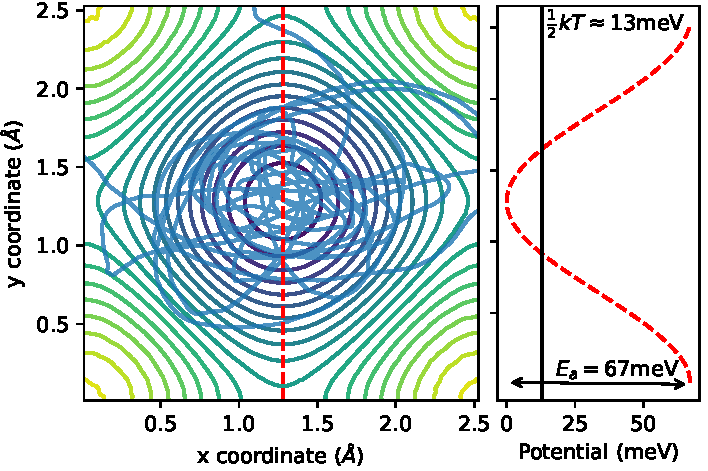
\includegraphics[width=1.0\columnwidth]{pot_surface}
	\caption{The potential energy surface extracted from the sodium on copper(001) 3D molecular dynamics simulation with a superimposed trajectory typical for a low friction activated diffusion process. The red dashed line in the right panel shows a cross-section of the potential through an adsorption site and two bridge sites as annotated in the panel on the left. All ISFs presented in this paper are quoted with the a momentum transfer pointing from the adsorption site through one of the equivalent bridge sites}
	\label{fig:pot_surface}
\end{figure}

\begin{figure}
	\centering
	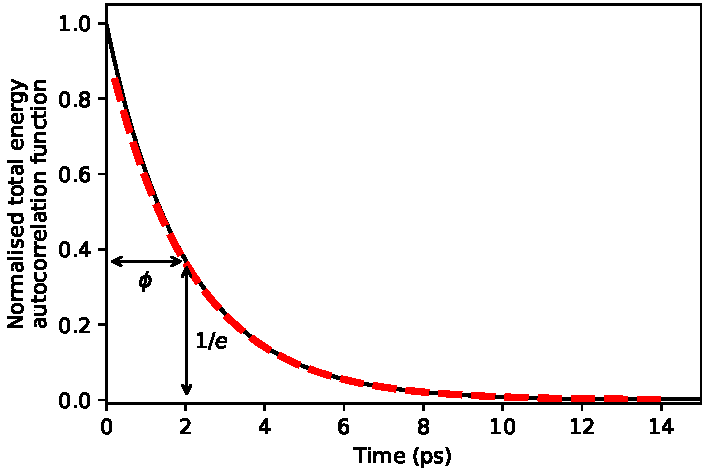
\includegraphics[width=1.0\columnwidth]{e_auto}
	\caption{The generalized energy exchange rate, $\phi^{-1}$, is defined as the inverse correlation time of the normalized total energy autocorrelation function. Since the total energy auto-correlation function is generally not a pure exponential, $\phi$ is defined as the time taken for the function to fall by a factor of $\frac{1}{e}$.}
	\label{fig:e_auto}
\end{figure}

\section*{Hopping rates}

\begin{figure}
	\centering
	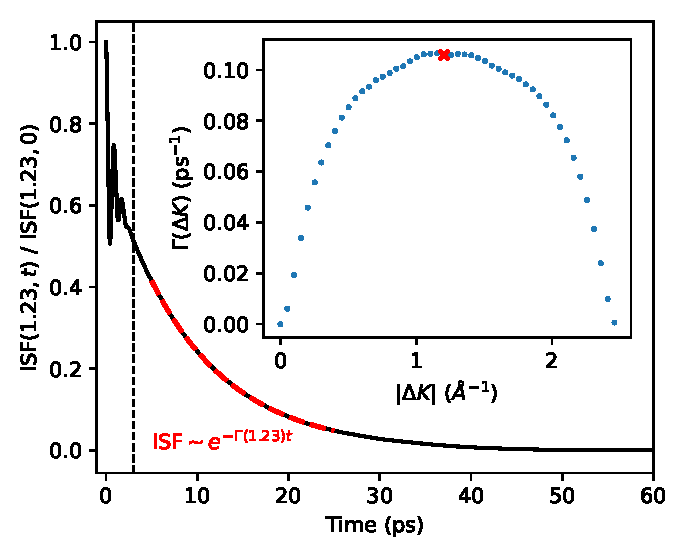
\includegraphics[width=1.0\columnwidth]{isf_dk}
	\caption{The main axes show a typical ISF over time for a fixed momentum transfer. The decay rate, $\Gamma$, of the ISF's exponential tail is proportional to the hopping rate of the adatom. By calculating $\Gamma$ over a range of momentum transfers, a jump distribution plot may be constructed as shown in the inset axes. The shape of the jump distribution is set by the distribution of adatom jump lengths.} 
	\label{fig:isf_dk}
\end{figure}

Each simulation was run repeatedly at $300\K$ for a total run time of up to $2\us$ per configuration. The hopping behavior of each simulated adatom was evaluated using the observable quantity in a surface scattering experiment, the intermediate scattering function,
$$
\mathrm{ISF}(\Delta{\vec{K}}, t) = \left<\exp\left(i\Delta{\vec{K}}\cdot\vec{r(t)}\right)\right>.
$$
A typical ISF for a fixed momentum transfer, $\Delta{\vec{K}}$, is shown in the main axes of Fig. \ref{fig:isf_dk}. In the case of activated diffusion, the long time decay rate of the ISF, $\Gamma$, is proportional to the adatom hopping rate, and the shape of $\Gamma$ as a function of $\Delta{K}$, as shown in the inset of Fig. \ref{fig:isf_dk}, is set by the distribution of jump lengths.

\begin{figure}
	\centering
	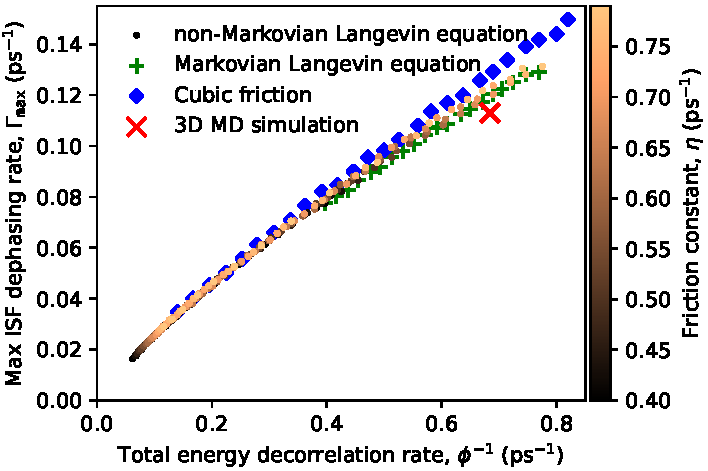
\includegraphics[width=1.0\columnwidth]{gamma_ttf}
	\caption{A scatter of the maximum ISF dephasing rate, $\Gamma_{\text{max}}$, against the energy exchange rate, $\phi^{-1}$, for each model demonstrates that the ISF dephasing rate is set by the energy exchange rate and the 2D potential background. Other microscopic details account for less than $3\%$ of the variance in the limit of low energy exchange rate. The color of the non-Markovian model's small points show the value of $\eta$ used in the simulation.}
	\label{fig:gamma_ttf}
\end{figure}

\begin{figure}
	\centering
	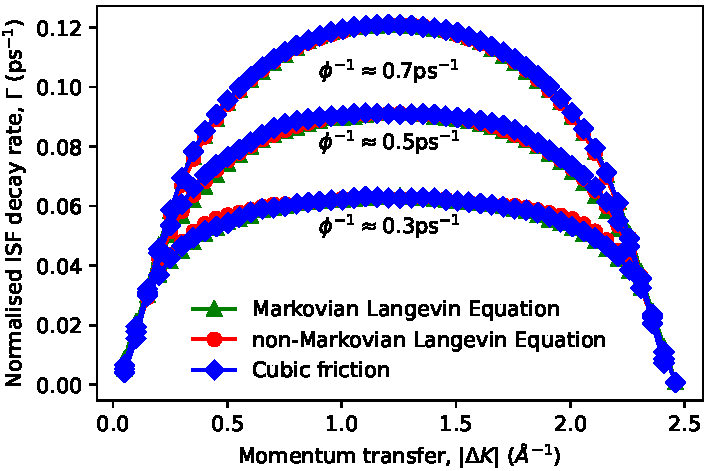
\includegraphics[width=1.0\columnwidth]{jump_distribution}
	\caption{Each set of points show the jump distribution of a particular model for three energy exchange rates: $\phi^{-1}=0.3$, $0.5$ and $0.7\ips$. A noise correlation time of $\tau=0.1\ps$ was used for the non-Markovian model in each instance. The jump distributions show very little variation across the models at a fixed energy exchange rate.} 
	\label{fig:jump_distribution}
\end{figure}

As a measure of the total hopping rate, The peak of the jump distribution, $\Gamma_{\text{max}}$ (annotated in Fig. \ref{fig:isf_dk}), was calculated for each model. The small round points in Fig. \ref{fig:gamma_ttf}, show that the energy exchange rate of the non-Markovian Langevin equation is an excellent estimator for the total hopping rate of the system. The color of the markers demonstrate that for fixed $\eta$, the total hopping rate can vary by many multiples when the noise correlation time is adjusted. However, when considered as a function of a fixed energy exchange rate, the hopping rate is found to vary by less than $3$\%. We therefore find that noise correlations do in fact have an effect on an adatom's hopping rate, however to first order, this effect only occurs through the energy exchange rate and can therefore be compensated for through an adjustment of $\eta$. The cubic model's hopping rate was found to vary linearly as a function of the coupling $\zeta$, however, if the energy exchange rate is tuned to match the exchange rate of the linear friction models, the hopping rate is found to lay within a few percent of the linear friction models. The 3D model was also found to lay within $6$\% of the Markovian Langevin simulation with an analogous energy exchange rate. 

The shape of the jump distribution of each model was compared by tuning the available parameters to run each model over a fixed set of energy exchange rates. The jump distributions for each model at the energy exchange rate of approximately $0.3$, $0.5$, and $0.7\ips$ are shown in Fig. \ref{fig:jump_distribution}. Since the variation of amplitudes is quantified in Fig. \ref{fig:gamma_ttf}, the jump distributions presented are normalized to peak at the same height within each energy transfer rate to allow for the comparison of the jump distribution shape. For a fixed energy exchange rate, the adatom jump distribution shapes were found to agree well across all models with only small differences in shape. The peaks of the jump distributions at higher exchange rates are all observed to be narrower than those at lower exchange rates, indicating an increase in the probability of single hops to adjacent sites\cite{Diamant}. This is expected as higher energy exchange rates decrease the probability that a particle which has escaped its well finds another bridge site before attaining an independent energy level, likely lower than the activation energy, and being bound to an adjacent well. The largest deviation is seen in the 3D model with a greater proportion of adatom jumps terminating outside of the adjacent adsorption sites compared to the 2D models.  

We therefore conclude that the hopping rate and jump distribution of a low-friction activated diffusion model are fixed by the 2D potential energy surface and the energy exchange rate, with almost complete independence of any other details in the low exchange rate limit. The deviations of the 3D model are not well understood but are likely due to additional memory effects as a result of energy exchange with the third co-ordinate and the 3D details of the potential affecting the probability of escape when enough energy is obtained. Furthermore the deviations seen across the board are well within the accuracy of current experimental techniques and therefore would not be observable within an experimental context (Would you be comfortable making this statement John? From what I can tell the accuracy of HSEM measurements around $\Gamma_{max}$ appears to be $\sim 10$\%.).

\section*{Energy exchange rates}

\begin{figure*}
	\centering
	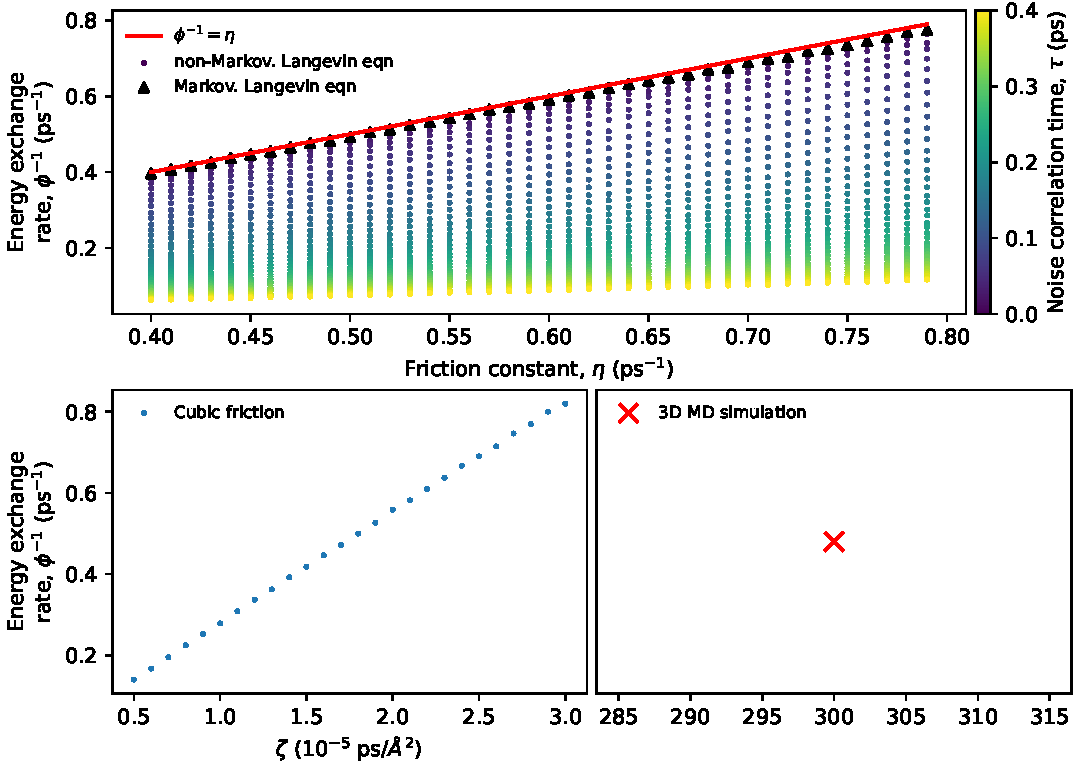
\includegraphics[width=0.8\textwidth]{energy_exchange_rates}
	\caption{Panel a) presents the variation of the energy exchange rate as a function of the friction parameter, $\eta$, and noise correlation time, $\tau$, in the linear friction Langevin models. The suppression factor, $I=\phi^{-1}/\eta$, of the non-Markovian Langevin model is shown in the b) alongside the suppression factor of an equivalent harmonic potential. The power spectrum of the force seen by an adatom held fixed at the minimum of an adsorption site in the 3D simulation is shown in c) inset with the corresponding time domain auto-correlation function. The energy exchange rate of the non-linear friction model as a function of the cubic friction coupling constant $\zeta$ is found in panel d).} 
	\label{fig:energy_exchange_rates}
\end{figure*}

Having established the generalized energy exchange rate as a quantity of interest, we shift focus to evaluating the effects which contribute to $\phi^{-1}$. The introduction of noise correlations was found to suppresses the energy exchange rate with the substrate, as shown in Fig. \ref{fig:energy_exchange_rates}a. For the sake of comparison, the red line shows the energy exchange rate of a particle with Markovian Langevin statistics in a harmonic well, $\phi^{-1}=\eta$. For short correlation times, we find the energy exchange rate is close to $\eta$, but even for $\tau=0$, there are small differences due to anharmonicities in the background potential. As the noise correlation time approaches $0.4\ps$, the energy exchange rate is seen to fall by close to a factor of four, demonstrating that the narrowing of the noise power spectrum can have a large effect on the energy exchange rate. Regardless of the noise correlation time, the exchange rate was found to remain linear in $\eta$ suggesting that $\eta$ continues to act as an overall interaction strength parameter while $\tau$ controls the coupling strength to individual modes, suppressing interactions with high frequency modes. 

The linear dependence on $\eta$ inspires the introduction of a dimensionless, $\eta$ independent, suppression factor $I = \frac{\phi^{-1}}{\eta}$ which quantifies the suppression of energy exchange as a function of $\tau$. The suppression factor for the non-Markovian simulation is shown in Fig. \ref{fig:energy_exchange_rates}b alongside an analytically derived suppression factor of an equivalent particle in a harmonic well. The toy model, solved in the supplemental information, is found to admit a similar $\eta$ independent suppression factor in the low friction limit. The qualitative agreement of the suppression factors indicates a similar underlying origin albeit distorted through anharmonicities in the corrugated potential. The origin of the effect can be understood by considering the expected energy change of the adatom when subjected to a single noise impulse which decays in time as $K(t)$. Without loss of generality, we suppose the impulse is imparted in the direction of the instantaneous velocity. If $K(t)$ decays quickly compared to the oscillation period, then the impulse is imparted entirely in the direction of motion, and the adatom quickly settles into a new, higher energy level. If $K(t)$ decays at a rate comparable to the oscillation period of the well then some of the energy imparted initially is removed when the force acts against the direction of motion as the adatom swings back. The new energy level attained is therefore not as high as in the former case and we expect a lower change in the total energy per impulse. A similar argument can be made for the correlated friction force removing less energy per oscillation. This interpretation is reflected in the mathematical form of the low friction approximation of the harmonic well's suppression factor as an oscillating integral over $K(t)$,
\begin{equation}
	I(\tau, \omega_0) = \int_0^{\infty}\diff{t}K(t)\cos{\omega_0t} = \mathrm{Re}\left(\tilde{K}(\omega_0)\right) = \frac{1}{1+\left(\omega_0\tau\right)^2}.
	\label{eq:suppression_factor}
\end{equation}
For an exponential memory kernel, the suppression factor coincides exactly with the power spectrum of the memory kernel, however in general this is not the case. 

Moreover, the power spectrum of noise in a physical system is likely to exhibit a much sharper cutoff than the Lorentzian spectrum of an exponential memory kernel. Fig. \ref{fig:energy_exchange_rates}c contrasts the power spectrum of the force experienced by an adatom held fixed at an equilibrium point of the 3D simulation compared to the Lorentzian spectrum used in our non-Markovian simulations. This spectrum is feature rich but clearly demonstrates a sharp cutoff around the copper cutoff frequency of $7.4\THz$. The corresponding time domain correlation function contains clear oscillations on the order of a few terahertz. By tuning the mass of the adatom in this simulation, a doubling in the energy exchange rate has been observed in the 3D simulation when the frequency of the noise correlation oscillations match those of the adatom. This effect warrents its own investigation but is included here to demonstrate that this effect is likely meaningful in the context of realistic phonon-adatom interactions. High atomic mass substrates such as lead or rubidium paired with light adatoms may result in the conditions needed to see this effect although it is unknown whether the effect would be visible over the other differences in such materials.

The energy exchange rate of the cubic friction model, shown in Fig. \ref{fig:energy_exchange_rates}d is included for completeness and was found to be linear in $\zeta$, with energy exchange rates comparable to the linear friction models when $\zeta$ is on the order of $10^{-5}\uzeta$. 


\section*{Discussion}

We conclude that the single energy exchange rate parameter obtained through the Markovian Langevin equation is sufficient for describing the transport properties of low friction activated surface diffusion. However, the energy exchange rate must be interpreted as an aggregation of subtle microscopic details, the breakdown of which may not be knowable. Although the ability to fit data with sophisticated microscopic statistics using a Markovian Langevin equation is an interesting result in its own right, the true goal is to construct models which can make causal predictions of surface processes. The most important determinants of the rate of chemical reactions on a surface are the distribution of reagents in phase space and the rate of replenishment of spent reagents. The results presented demonstrate that a Markovian Langevin equation equipped with the correct energy exchange rate gets precisely this right. For simple monatomic species, this is the end of the story and the Markovian Langevin equation can likely be safely used for the prediction of surface processes. We however make the final comment that the reactions of larger molecules is influenced by their conformational mobility. Kramer's theory of reaction rates\cite{Kramers, Zwanzig} treats the contortion of molecules as a diffusive process in its own right, driven by Markovian noise\cite{Kramers, Zwanzig}. While the timescale of most molecular vibrations is much greater than the phonon cutoff frequency of a substrate, there are examples of certain molecular vibrational modes, in Benzene for example\cite{Wang2020}, which fluctuate as slowly as $10\THz$. If these vibrational modes are important to the rate of a particular reaction, the details of a substrate's phonon spectrum may become relevant. 

%TC:ignore
\section*{Methods}

\subsection*{Langevin simulations}

The 2D Langevin simulations were performed with a $\Delta{t} = 1\fs$ timestep for a total of $2\us$ of simulation run time spread over $200$ separate $10\ns$ trajectories. At each timestep, the background force on the adatom was determined through the gradient of the background potential, as interpolated using a bicubic spline on the $100\times100$ grid provided in the Supplemental Information. The random force was sampled independently for each force component from a zero-mean gaussian random variable with standard deviation $\sigma/\sqrt{\Delta{t}}$ where the relevant fluctuation dissipation theorem sets $\sigma$ through $\left<f\left(t_1\right)f\left(t_2\right)\right>=\sigma^2\delta\left(t_1-t_2\right)$. Convolution with a discretized exponential memory kernel was performed through the relation
$$
\int_0^{t_n} dt' K\left(t-t'\right) \vec{f}(t') \approx \alpha \int_0^{t_{n-1}} dt' K\left(t-t'\right) \vec{f}(t') + \frac{1}{1-\alpha} \vec{f}\left(t_n\right)
$$
where $\alpha = \exp{\frac{-\Delta{t}}{\tau}}$. The coloured noise spectrum was produced by generating an uncorrelated sequence of impulses and convolving with $K(t)$, this trick is only valid for an exponential memory kernel. Once the net force was determined as the sum of the background force, noise force, and the relevant friction law, the adatom position and velocity were propegated forwards in time using a Velocity-Verlet integrator\cite{Verlet}.

\subsection*{3D molecular dynamics simulations}

The 3D molecular dynamics simulation was constructed in a similar fashion to the simulation constructed by Ellis\cite{Ellis} and used the same substrate spring constant and Morse potential parameters. The key difference is that a larger $8\times8\times8$ substrate was used and the pairwise adatom interactions with the substrate atoms were tracked up to a separation of $3.1$ times the Morse potential parameter $r_0$ in separation. A Velocity Verlet integrator\cite{Verlet} with a $10\fs$ timestep was used to propegate the simulation through time for $200$ runs of $10\ns$ at $300\K$.

\subsection*{Extracting the 2D background potential}

The 3D MD simulation was used to produce $2\us$ of adatom trajectory at 8 temperatures across the range $140-300\K$. The $2\us$ trajectory of each temperature was mapped back into the first 2D unit cell on the periodic surface and binned into a $100\times100$ 2D grid. Using Eq. \ref{eq:free_energy}, the 2D free energy was calculated and verified not to vary as a function of temperature. The potential grid provided in the supplemental information and shown in Fig. \ref{fig:pot_surface} is the arithmatic mean of these grids.

\section*{Code availability}

All code was written in a combination of Python and Cython and is available on github through the link \url{https://github.com/jjhw3/gle_research}. If this manuscript is accepted for publication I will provide a condensed version of the code as this repository was used for many projects relating to Langevin and Molecular Dynamics simulations and therefore contains some clutter. 

\section*{Data availability}

The trajectories of all 3D molecular dynamics simulations is available upon request. The trajectories of Langevin simulations were not stored due to storage space constraints (The equivelant of more than 20Tb of data in total), however, equivelant trajectories may be readily simulated in two days. The total energy autocorrelation function of each Langevin simulation run was stored and these are available upon request. The microcanonical ensemble average of the first $100\ps$ of these autocorrelation functions is provided in the supplemental information.

\bibliography{bibliography}

\pagebreak
\onecolumn

\section*{Supplemental Information}

\subsection*{The Langevin potential energy surface}

Attached as text file.

\subsection*{Exchange rate data for Fig. \ref{fig:energy_exchange_rates}}

The first $20\ps$ of the total energy autocorrelation function of each simulation is provided as an xlsx file.

\subsection*{ISF decay rate for each simulation in Fig. \ref{fig:gamma_ttf}}

The jump distributions of each simulation shown in Fig. \ref{fig:gamma_ttf} is provided as an xlsx file.

\subsection*{The jump distributions in Fig. \ref{fig:jump_distribution}}

The jump distributions and simulation parameters used to generate Fig. \ref{fig:jump_distribution} are provided as an xlsx file.


\subsection*{Energy exchange rate of the 3D simulation}

\begin{figure*}
	\centering
	\includegraphics[width=0.5\textwidth]{MD_e_auto}
	\caption{The total energy autocorrelation function of the 3D simulation shows an extremely fast drop at short times not present in 2D simulations. This is assumed to be caused by fast motion in the perpendicular co-ordinate. To compensate for this, the decay rate of the tail is used as the energy exchange rate for this simulation.} 
	\label{fig:MD_e_auto}
\end{figure*}

There is a certain ambiguity as to what energy to use for the definition of the energy exchange rate of the 3D simulation. Although energy may be exchanged with the third co-ordinate, the motion in the this direction is generally much faster than in the lateral directions. This leads to undesireable oscillations in the total energy auto-correlation function if one tries to use a definition in terms of the lateral co-ordinates only. Subsequently, we decided to use the 3D total energy of the adatom as the sum of its kinetic energy in all three dimensional plus the free energy as a function of all three co-ordinates. The 3D free energy was determined in the same fashon described in the methods section except the position was binned on a 3D grid. The resulting total energy autocorrelation function, Fig. \ref{fig:MD_e_auto}, contains an extremely fast drop at short times not present in 2D simulations. This is assumed to be caused by fast motion in the perpendicular co-ordinate. To compensate for this, the decay rate of the tail is used as the energy exchange rate for this simulation. An investigation into how to rigorously define effective 2D properties from such 3D simulations is a potential avenue for future work.

\section*{Derrivation of the suppresion factor for a particle in a harmonic well with non-Markovian noise}

\begin{figure*}
	\centering
	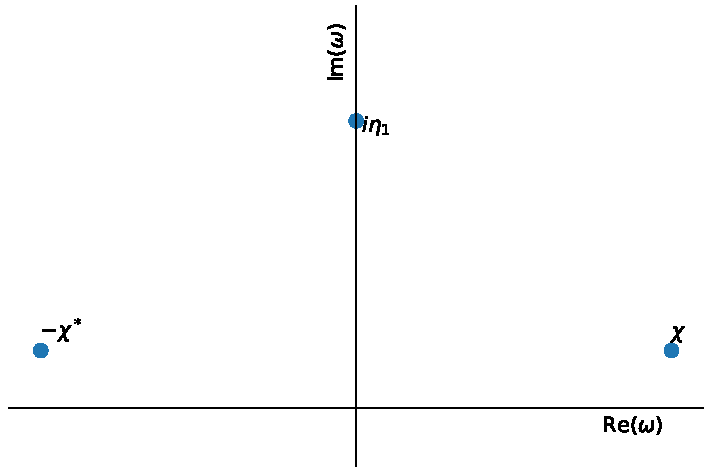
\includegraphics[width=0.5\textwidth]{F_poles}
	\caption{The pole structure of the Green's function of the non-Markovian Langevin equation with an exponential memory kernel.} 
	\label{fig:F_poles}
\end{figure*}

The non-Markovian Langevin equation in a harmonic well of natural frequency $\omega_0$ is given by
$$
	m\ddot{\vec{r}}+m\eta\int\diff{t'}K(t-t')\dot{\vec{r}}(t')+m\omega_0^2\vec{r}=\vec{f}(t)
$$
$$
	\text{ where } \left<f(t_1)f(t_2)\right>=2k_BTm\eta K(\left|t_1-t_2\right|).
$$
where $K(t)$ is a causal memory kernel with total area of $1$. Taking the Fourier transform of this equation, applying the convolution theorem, and collecting terms results in a solution for the particle's trajectory in Fourier space in terms of a Green's function $\tilde{F}$,
\begin{equation}\label{eq:greens_function}
	\tilde{x} = \frac{1}{m} \frac{\tilde{f}}{-\omega^2 + i \eta \omega \tilde{K} + \omega_0^2} = \frac{1}{m} \tilde{f} \tilde{F} 
\end{equation}
$$
\implies x(t) = \frac{1}{m}\int\frac{\diff{\omega}}{2\pi}\tilde{f} \tilde{F} e^{i\omega t}.
$$
The ensemble average of observables like the energy exchange rate, $\phi^{-1}$, are functions of the positions of the poles of $\tilde{F}$. Although the introduction of $\tilde{K}$ will in general add further poles to the Green's function, the residue of the two poles evident in the denominator of Eq. \ref{eq:greens_function} are the dominant features of the total energy autocorrelation function. In particular, it may be shown that in the low friction limit, the energy exchange rate is given by twice the imaginary co-ordinate of these poles. We therefore evaluate the energy exchange rate of the system through the shift of these two poles as a result of $\tilde{K}$ by factorizing the denominator in Eq. \ref{eq:greens_function},
$$
\frac{1}{-\omega^2 + i \eta \omega \tilde{K} + \omega_0^2} = \frac{-1}{\left(\omega - \frac{i\eta\tilde{K}}{2} + \omega_0\sqrt{1-\left(\frac{i\eta\tilde{K}}{2\omega_0}\right)^2}\right)\left(\omega - \frac{i\eta\tilde{K}}{2} - \omega_0\sqrt{1-\left(\frac{i\eta\tilde{K}}{2\omega_0}\right)^2}\right)}
$$
We proceed by labelling one of the poles $\chi$ and suppose it satisfies
$$
\left(\chi - \frac{i\eta\tilde{K}(\chi)}{2} - \omega_0\sqrt{1-\left(\frac{i\eta\tilde{K}(\chi)}{2\omega_0}\right)^2}\right)=0.
$$
First we note that $\chi=\omega_0$ for $\eta=0$ and proceed by expanding $\chi$ to the lowest order in $\eta$. Implicitly differentiating the above expression with respect to $\eta$ and taking $\eta=0$ demonstrates that $\chi = \omega_0 + \frac{i\eta\tilde{K}(\omega_0)}{2} + O(\eta^2)$. Therefore in the low friction limit, the imaginary component of $\chi$ is shifted to $\frac{\eta\operatorname{Re}(\tilde{K}(\omega_0))}{2}$ and the suppression factor is given by $I=\frac{\phi^{-1}}{\eta}=\frac{2\operatorname{Im}(\chi)}{\eta}=\operatorname{Re}(\tilde{K}(\omega_0))$. In the case of a causal exponential memory kernel with correlation time $\tau$, this gives $I=\frac{1}{1+(\omega_0\tau)^2}$ 


\subsection*{Exact analytic expressions for the ISF and kinetic energy autocorrelation function of a particle in a harmonic well with non-Markovian noise}

Do you think it is worth cleaning this up and including it in the submission (lines 560-600)? Its interesting and useful to me, but I'm not sure whether anyone else will ever use it.

The non-Markovian Langevin equation in a harmonic well of natural frequency $\omega_0$ is given by
$$
m\ddot{\vec{r}}+m\eta\int\diff{t'}K(t-t')\dot{\vec{r}}(t')+m\omega_0^2\vec{r}=\int\diff{t'}\vec{f}(t')K(t-t')
$$
where $K(t)$ is a causal memory kernel with total area of $1$. Taking the Fourier transform of this equation, applying the convolution theorem, and collecting terms results in a solution for the particle's trajectory in Fourier space in terms of a Green's function $\tilde{F}$,
$$
\tilde{x} = \frac{1}{m} \frac{\tilde{f} \tilde{K}}{-\omega^2 + i \eta \omega \tilde{K} + \omega_0^2} = \frac{1}{m} \tilde{f} \tilde{F}. \label{eq:greens_function}
$$
In the case of a causual exponential memory kernel $K(t)=\frac{1}{\tau}e^{-\frac{t}{\tau}}$, with Fourier spectrum $\tilde{K}(\omega)=\frac{1}{1+i\omega\tau}$, the Green's function is the reciprocal of a third order polynomial,
$$
\tilde{F} = \frac{-1}{i\tau\omega^3 + \omega^2 - i\omega(\omega_0^2\tau + \eta) - \omega_0^2} =: \frac{-1}{P(\omega)}.
$$
Since $P(i\omega)$ is a polynomial with real co-efficients, it follows from the complex conjugate root theorem that for any root $z$ of $P(\omega)$, $-z^*$ is also a root of $P(\omega)$. This allows us to make the ansatz that $P$ may be factorized as $P(\omega) = i\tau\left(\omega - \chi\right)\left(\omega + \chi^*\right)\left(\omega - i\eta_1\right)$ for some $\chi\in\mathbb{C}$ and ${\eta_1\in\mathbb{R}}$. While it is possible that $P(\omega)$ admits three imaginary solutions in some regions of the $\tau,\eta,\omega_0$ parameter space, these parameter ranges have not been encountered in our study of activated diffusion. If the Greens function $F(t)$ is to be causal, all three roots must occur in the upper half plane. We therefore find that the pole structure of $\tilde{F}(\omega)$ is of the form shown in Figure \ref{fig:F_poles}. A simple application of the residue theorem allows useful integrals of the form $\int\frac{dw}{2\pi} g\left(\omega\right) \left|\tilde{F}\left(\omega\right)\right|^2$ to be evaluated using the formula,


The non-Markovian Langevin equation in a harmonic well of natural frequency $\omega_0$ is given by
$$
m\ddot{\vec{r}}+m\eta\int\diff{t'}K(t-t')\dot{\vec{r}}(t')+m\omega_0^2\vec{r}=\int\diff{t'}\vec{f}(t')K(t-t')
$$
where $K(t)$ is a causal memory kernel with total area of $1$. Taking the Fourier transform of this equation, applying the convolution theorem, and collecting terms results in a solution for the particle's trajectory in Fourier space in terms of a Green's function $\tilde{F}$,
$$
\tilde{x} = \frac{1}{m} \frac{\tilde{f} \tilde{K}}{-\omega^2 + i \eta \omega \tilde{K} + \omega_0^2} = \frac{1}{m} \tilde{f} \tilde{F}. \label{eq:greens_function}
$$
In the case of a causual exponential memory kernel $K(t)=\frac{1}{\tau}e^{-\frac{t}{\tau}}$, with Fourier spectrum $\tilde{K}(\omega)=\frac{1}{1+i\omega\tau}$, the Green's function is the reciprocal of a third order polynomial,
$$
\tilde{F} = \frac{-1}{i\tau\omega^3 + \omega^2 - i\omega(\omega_0^2\tau + \eta) - \omega_0^2} =: \frac{-1}{P(\omega)}.
$$
Since $P(i\omega)$ is a polynomial with real co-efficients, it follows from the complex conjugate root theorem that for any root $z$ of $P(\omega)$, $-z^*$ is also a root of $P(\omega)$. This allows us to make the ansatz that $P$ may be factorized as $P(\omega) = i\tau\left(\omega - \chi\right)\left(\omega + \chi^*\right)\left(\omega - i\eta_1\right)$ for some $\chi\in\mathbb{C}$ and ${\eta_1\in\mathbb{R}}$. While it is possible that $P(\omega)$ admits three imaginary solutions in some regions of the $\tau,\eta,\omega_0$ parameter space, these parameter ranges have not been encountered in our study of activated diffusion. If the Greens function $F(t)$ is to be causal, all three roots must occur in the upper half plane. We therefore find that the pole structure of $\tilde{F}(\omega)$ is of the form shown in Figure \ref{fig:F_poles}. A simple application of the residue theorem allows useful integrals of the form $\int\frac{dw}{2\pi} g\left(\omega\right) \left|\tilde{F}\left(\omega\right)\right|^2$ to be evaluated using the formula,
\begin{equation}
	\int\frac{dw}{2\pi} g\left(\omega\right) \left|\tilde{F}\left(\omega\right)\right|^2 =  -\frac{1}{2 \tau^{2}}\left(\frac{1}{2 \chi' \chi''} \operatorname{Re}\left(\frac{g(\chi)}{\chi\left(\chi^{2}+\eta_{1}^{2}\right)}\right)+\frac{g(i\eta_{1})}{\left(|\chi|^{2}+n_{1}^{2}\right)^{2} \eta_{1}}\right), \label{eq:integral_over_CF}
\end{equation}
provided $g(\omega)$ is an entire function which decays sufficiently fast as $\operatorname{Im}({\omega})\rightarrow\infty$.

\subsection*{Evaluating the ISF}

The intermediate scattering function is given by the spatial Fourier transform of the van Hove pair correlation function $G\left(\vec{r},t\right)$. For a single particle, this is equivalent to $P\left(\vec{r}, t\right)$, the probability of finding the particle at $\vec{r}$ at time $t$ given that it was at the origin at $t=0$. For a single particle trajectory, $\vec{r}(t)$, this given by 

$$
ISF(\Delta \vec{K}, t) = \int d\vec{R} e^{-i \Delta \vec{K} \cdot \left(\vec{R} - \vec{r}(0)\right)} P(\vec{R}, t) = \int d\vec{R} e^{-i \Delta \vec{K} \cdot \left(\vec{R} - \vec{r}(0)\right)} \delta(\vec{R} - \vec{r}(t)) = e^{-i \Delta \vec{K} \cdot \left(\vec{r}(t) - \vec{r}(0)\right)}
$$
\\
Inserting the solution for $\vec{r}(t)$ in terms of the Green's function, expanding the exponential and taking an ensemble average gives
$$
\left<ISF(\Delta \vec{K}, t)\right> = \sum_{n=0}^{\infty} \left(- \frac{i}{m}\right)^n \frac{1}{n!} \left< \left( \int \frac{d\omega}{2\pi} \left(e^{i\omega t} - 1\right) \tilde{F} \left(\Delta \vec{K} \cdot \tilde{f}\right)\right)^n\right>
$$
\\
\begin{equation}
= \sum_{n=0}^{\infty} \left(- \frac{i}{m}\right)^n \frac{1}{n!} \left( \int \frac{d\omega}{2\pi} \left(e^{i\omega t} - 1\right) \tilde{F}\right)^n \left< \left(\Delta \vec{K} \cdot \tilde{f}\right)^n\right> \label{eq:isf_1}
\end{equation}
\\
I have abused notation in the last line to summarize $n$ integrals over $\omega_1$ through $\omega_n$. Taking a closer look at $\left< \left(\Delta \vec{K} \cdot \tilde{f}\right)^n\right>$ in one dimension,
$$
\left< \left(\Delta \vec{K} \cdot \tilde{f}\right)^n\right> = \left|\Delta \vec{K}\right|^n \left< \tilde{f}\left(\omega_1\right) \ldots \tilde{f}\left(\omega_n\right)\right>.
$$
From the isotropy and zero mean of $f$ it follows that the above vanishes for odd $n$. Assuming $f$ is a gaussian random variable, expectation value for even $n$ is given by the sum over the product of all possible pairwise expectations of $\left< \tilde{f}\left(\omega_1\right) \ldots \tilde{f}\left(\omega_n\right) \right>$,
$$
\left< \left(\Delta \vec{K} \cdot \tilde{f}\right)^{2n}\right> = \left|\Delta \vec{K}\right|^{2n} \frac{1}{2^nn!} \sum_P \left< \tilde{f}\left(\omega_{P_1}\right) \tilde{f}\left(\omega_{P_2}\right)\right> \ldots \left< \tilde{f}\left(\omega_{P_{2n-1}}\right) \tilde{f}\left(\omega_{P_{2n}}\right)\right>
$$
$$
= \left|\Delta \vec{K}\right|^{2n} \frac{\left(2\pi\sigma^2\right)^n}{2^nn!} \sum_P \delta\left(\omega_{P_1} + \omega_{P_2}\right) \ldots \delta\left(\omega_{P_{2n-1}} + \omega_{P_{2n}}\right)
$$
The last step follows immediately from the Fourier transform of $\left<f(t)f(t')\right>=\delta(t-t')\sigma^2$. Substituting into \ref{eq:isf_1} yields
$$
\sum_{n=0}^{\infty} \left(- \frac{i}{m}\right)^{2n} \frac{1}{(2n)!} \left( \int \frac{d\omega}{2\pi} \left(e^{i\omega t} - 1\right) \tilde{F}\right)^{2n} \left|\Delta \vec{K}\right|^{2n} \frac{\left(2\pi\sigma^2\right)^n}{2^nn!} \sum_P \delta\left(\omega_{P_1} + \omega_{P_2}\right) \ldots \delta\left(\omega_{P_{2n-1}} + \omega_{P_{2n}}\right)
$$
$$
= \sum_{n=0}^{\infty} \left(- \frac{i}{m}\right)^{2n} \frac{1}{(2n)!} \left( \int \frac{d\omega}{2\pi} \left|\left(e^{i\omega t} - 1\right) \tilde{F}\right|^2\right)^{n} \left|\Delta \vec{K}\right|^{2n} \frac{\left(\sigma^2\right)^n(2n)!}{2^nn!}
$$
$$
= \sum_{n=0}^{\infty} \frac{1}{n!} \left(-\frac{|\Delta \vec{K}|^2 \sigma^2}{m^2} \int \frac{d\omega}{2\pi}\left(1 - \cos\left(\omega t\right)\right) \left| \tilde{F} \right|^2\right)^n
$$
\begin{equation}
= \exp\left(-\frac{|\Delta \vec{K}|^2 \sigma^2}{m^2} \int \frac{d\omega}{2\pi}\left(1 - \cos\left(\omega t\right)\right) \left| \tilde{F} \right|^2\right) \label{isf_explicity_norm}
\end{equation}
\\
From equation \ref{isf_explicity_norm} it is clear the ISF is normalized to 1 at $t=0$. Since $F(t)$ is a real function, $|\tilde{F}|^2$ must be even, so $\int \frac{d\omega}{2\pi}\left(\cos\left(\omega t\right)\right) \left| \tilde{F} \right|^2 = \int \frac{d\omega}{2\pi}\ e^{i \omega t} \left| \tilde{F} \right|^2$ which is nothing but the auto-correlation of $F(t)$. This integral may be evaluated using Eq. \ref{eq:integral_over_CF} resulting in the final expression, 
\begin{equation}
	ISF\left(\Delta \vec{K}, t\right) = ISF\left(\Delta \vec{K}, \infty\right) \exp\left(\frac{-\sigma^2\left|\Delta \vec{K}\right|^2}{2m^2\tau^2}\left(\frac{e^{-\chi''t}}{2\chi'\chi''}\operatorname{Re}\left(\frac{e^{i\chi't}}{\chi\left(\chi^2+\eta_1^2\right)}\right) + \frac{e^{-\eta_1t}}{\left(\left|\chi\right|^2+\eta_1^2\right)^2\eta_1}\right)\right) \label{isf_exp}.
\end{equation}

This expression is extremely useful as the starting point for certain short-time theoretical calculations and for checking the correctness of computational work.

\subsection*{Evaluating the kinetic energy autocorrelation function}

The velocity the particle may be written in terms of the Green's function as $\dot{x}(t) = \frac{i}{m}\int\frac{d\omega}{2\pi} \omega e^{i\omega t}\tilde{f}(\omega)\tilde{F}(\omega)$. The kinetic energy auto-correlation function is therefore given by
$$
\left<E(0)E(t)\right>=\frac{m^2}{4}\left<\dot{x}(0)^2\dot{x}(t)^2\right>=\frac{1}{4m^2}\left(\int\frac{d\omega}{2\pi}\omega\tilde{F}\right)^4 e^{i\left(\omega_3 + \omega_4 \right)t} \left<\left(\tilde{f}(\omega_1)\cdot\tilde{f}(\omega_2)\right)\left(\tilde{f}(\omega_3)\cdot\tilde{f}(\omega_4)\right)\right>.
$$
I have once again abused notation to summarize four integrals over $\omega_1\cdots\omega_4$. By expanding the dot product component wise and taking care to sum over all the products of pairwise expectations,  $\left<\left(\tilde{f}(\omega_1)\cdot\tilde{f}(\omega_2)\right)\left(\tilde{f}(\omega_3)\cdot\tilde{f}(\omega_4)\right)\right>$ is given by

$$
2\left(2\pi\sigma^2\right)^2\left(2\delta(\omega_1+\omega_2)\delta(\omega_3+\omega_4) + \delta(\omega_1+\omega_2)\delta(\omega_3+\omega_4) + \delta(\omega_1+\omega_2)\delta(\omega_3+\omega_4)\right).
$$
\\
Therefore in 2 dimensions,
$$
\left<E(0)E(t)\right>=\frac{\sigma^4}{m^2}\left(\left(\int\frac{dw}{2\pi}\omega^2\left|\tilde{F}(\omega)\right|^2\right)^2 + \left(\int\frac{dw}{2\pi}e^{i\omega t}\omega^2\left|\tilde{F}(\omega)\right|^2\right)^2\right).
$$
Which may be evaluated for an exponential memory kernel using Eq. \ref{eq:integral_over_CF} giving,

\begin{equation}
	\left<E(0)E(t)\right>=\left<E(0)E(\infty)\right> + \frac{\sigma^4}{4\tau^4m^2}\left(\frac{e^{-\chi''t}}{2\chi'\chi''}\operatorname{Re}\left(\frac{\chi e^{i\chi't}}{\chi^2+\eta_1^2}\right) + \frac{\eta_1e^{-\eta_1 t}}{\left(\left|\chi\right|^2 + \eta_1^2\right)^2} \right)^2 \label{eq:ek_auto}
\end{equation}
$$
\left<E(0)E(\infty)\right> = \frac{\sigma^4}{4\tau^4m^2}\left(\frac{1}{2\chi'\chi''}\operatorname{Re}\left(\frac{\chi}{\chi^2+\eta_1^2}\right) - \frac{\eta_1}{\left(\left|\chi\right|^2 + \eta_1^2\right)^2} \right)^2.
$$
The expression for $\left<E(0)E(\infty)\right>$ is particularly interesting as it is not exactly equal to $(k_BT)^2$, although in the relevant parameter range it is very close. This gives a tangible example of the temperature parameter used in the fluctuation dissipation relation giving an incorrect system temperature.

%TC:endignore

\end{document} 
